\begin{frame}
    \frametitle{Motivation}
    In the theory of stellar structures, the
    \alert{Lane-Endem equation}~(\cite{emden1907}~\Citeauthor{emden1907},~\citeyear{emden1907};
    \cite{lane1870}~\Citeauthor{lane1870},~\citeyear{lane1870}) has been used to describe the
    temperature variation in a star with hydrostatic equilibrium
    under a polytropic framework.

    \pause

    \begin{columns}[c] % [t] para alinear arriba
        \begin{column}{0.38\textwidth}
            \begin{figure}[ht!]
                \centering
                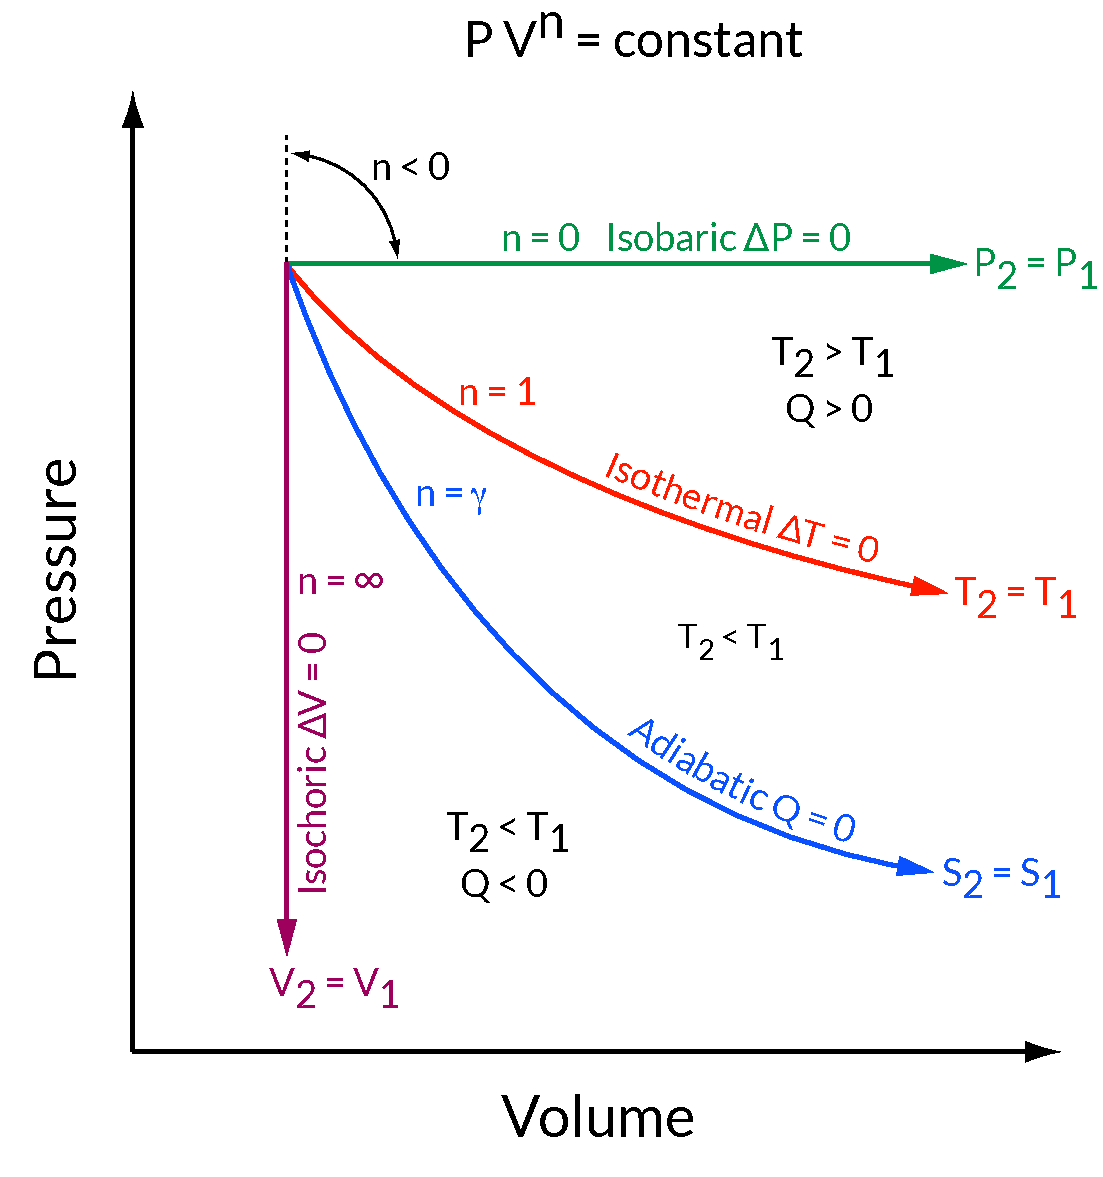
\includegraphics[width=.35\paperwidth]{pv_polytropic}
                \caption{Description.}
            \end{figure}
            %\cite{adomian1995} \cite{wazwaz}
        \end{column}
        \begin{column}{0.58\textwidth}
            The stellar model~\cite[p.~83]{maciel2007stellar}
            combines
            \begin{align}
                \diff{P\left(r\right)}{r} & =
                -\frac{GM\left(r\right)\rho\left(r\right)}{r^{2}}.
                \tag{Hydrostatic equilibrium condition} \\
                \diff{M\left(r\right)}{r} & =
                4\pi r^{2}\rho\left(r\right).
                \tag{Mass equation}                     \\
                P\left(r\right)           & =
                K{\left[\rho\left(r\right)\right]}^{1+\frac{1}{n}}.
                \tag{Polytropic equation of state}
            \end{align}
            %\cite{maciel2007stellar}
            %\cite{alzate2014}
            Where
            \begin{columns}
                \begin{column}{.23\paperwidth}
                    \begin{itemize}
                        \item $P\left(r\right)$: pressure function.
                        \item $\rho\left(r\right)$: density function.
                        \item $M\left(r\right)$: mass function.
                    \end{itemize}
                \end{column}
                \begin{column}{.26\paperwidth}
                    \begin{itemize}
                        \item $n$: polytropic index. % non-negative 
                        \item $K$: pressure constant. % positive
                        \item $G$: gravitational constant.
                    \end{itemize}
                \end{column}
            \end{columns}

            \

            These set of equations leads to the \alert{Lane-Endem equation}:
            \begin{equation*}
                \frac{1}{r^{2}}
                \diff*{\left[\frac{r^{2}}{\rho}\diff{P\left(r\right)}{r}\right]}{r}=
                -4\pi G\rho\left(r\right).
            \end{equation*}
        \end{column}
    \end{columns}
\end{frame}
\note{
    This equation is a consequence of hydrostatic equilibrium and pressure-density.
}
%https://link.springer.com/book/10.1007/978-3-662-70016-7 https://www.google.com/search?q=lane+emden+equation+derivation&client=firefox-b-d&sca_esv=b9fa5bd4402cbaee&biw=1536&bih=845&ei=WMAraYPxOruzkvQPsI6QuQE&ved=0ahUKEwiD_fW9_ZiRAxW7mYQIHTAHJBcQ4dUDCBE&uact=5&oq=lane+emden+equation+derivation&gs_lp=Egxnd3Mtd2l6LXNlcnAiHmxhbmUgZW1kZW4gZXF1YXRpb24gZGVyaXZhdGlvbjIHEAAYgAQYEzIFEAAY7wUyCBAAGIAEGKIEMgUQABjvBTIFEAAY7wVI-SFQLlj8BnABeAGQAQCYAfwDoAHbF6oBCTItMS40LjIuMbgBA8gBAPgBAZgCCaAC_RfCAgYQABgWGB6YAwCSBwkxLjAuMS40LjOgB6wesgcHMi0xLjQuM7gH-hfCBwUwLjQuNcgHGg&sclient=gws-wiz-serp  https://www.astro.physik.uni-potsdam.de/~htodt/ca/lane-emden.pdf https://link.springer.com/book/10.1007/978-1-4419-9110-2